\section{Scenario}
\label{sec:analysis:scenarios}

This section describes a scenario the envisioned system may be used in and outlines the target group of the system.

In \cite[p. 15]{prespecialisation} we defined the target group as people living in a smart home and interested in controlling the state of their home, \eg~lights, music centers, doors and windows, in a convenient matter. The group of people will currently consist of early adoptors of smart home technologies but based on the trend in IoT, our assumption is that the technology will be widespread within 5-10 years. 

We extend the definition of the target group presented in \cite[p. 15]{prespecialisation} to include a definition of the surroundings. As shown in \Cref{appendix:housing-types:table} the most common size of housings in Denmark is 75-99 square meters. Therefore we assume that the solution presented in this report is installed in a typical Danish apartment with a size of 90 square meters and with 3-4 rooms. 

We make the following assumptions about the system and the environment in which the scenario takes place:

\begin{itemize}
    \item All controllable devices are connected through a central hub.
    \item The system is installed in a private home where the different rooms can be defined.
    \item The state of the controllable devices is always available.
    \item The location of the user is always available when he is in his home.
\end{itemize}

We assume each room has two-three controllable lamps. The living room may have a television and a music center while the kitchen may have a controllable coffee machine. We estimate that 2-5 controllable devices per room seems fair leaving us with a maximum of 20 controllable devices in an apartment.

We consider the system to be installed in the apartment shown in \Cref{fig:analysis:scenario:apartment}. The rooms in the apartment are listed in \Cref{tbl:analysis:scenario:rooms} along with the controllable devices that seem realistic to be located in each room.

\begin{table}[h!]
\centering
\caption{Rooms in the apartment with possible devices in each room.}
\label{tbl:analysis:scenario:rooms}
\begin{tabular}{ll}
\textbf{Region} & \textbf{Controllable devices}                                                 \\
Hallway         & Two lamps and a door lock.                                                    \\
Living room     & Three lamps, a television, a music centre, a thermostat and a weather station.\\
Kitchen         & Two lamps, a coffee maker and a music centre.                                 \\
Bedroom         & Two lamps and a television.                                                   \\
Home office     & Two lamps and a music centre.                                                 \\
Bathroom        & A lamp.                                                                      
\end{tabular}
\end{table}

\Cref{tbl:analysis:scenario:gestures} shows the gestures a user may perform in the apartment shown in \Cref{fig:analysis:scenario:apartment}.

\begin{table}[h!]
\centering
\caption{Gestures the user has configured.}
\label{tbl:analysis:scenario:gestures}
\begin{tabular}{ll}
\textbf{Gesture name} & \textbf{Illustration}
\\[0.2cm]
Z                     &  
\begin{minipage}{.3\textwidth}
  
\includegraphics[height=1cm]{images/gesture-z}
\end{minipage}
\\[0.5cm]
V                     &
\begin{minipage}{.3\textwidth}
  
\includegraphics[height=1cm]{images/gesture-v}
\end{minipage}
\\[0.5cm]
Circle                &
\begin{minipage}{.3\textwidth}
  
\includegraphics[height=1cm]{images/gesture-circle}
\end{minipage}
\\[0.5cm]
Triangle              &
\begin{minipage}{.3\textwidth}
  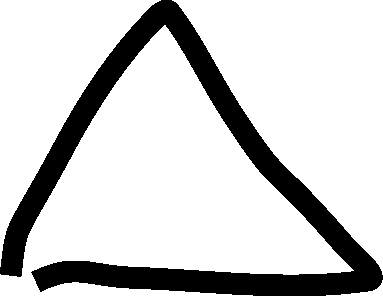
\includegraphics[height=1cm]{images/gesture-triangle}
\end{minipage}
\\[0.5cm]
L                     &
\begin{minipage}{.3\textwidth}
  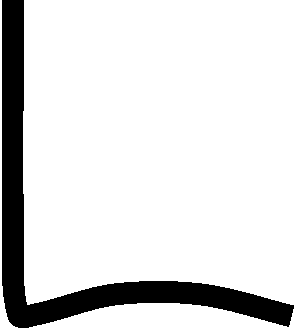
\includegraphics[height=1cm]{images/gesture-l}
\end{minipage}
\\[0.5cm]
W                     &
\begin{minipage}{.3\textwidth}
  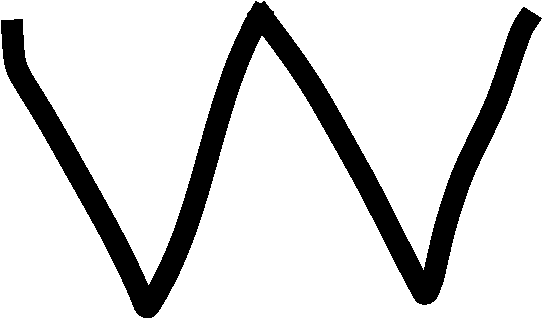
\includegraphics[height=1cm]{images/gesture-w}
\end{minipage}
\\[0.5cm]
Horizontal Line       &
\begin{minipage}{.3\textwidth}
  
\includegraphics[width=1.75cm]{images/gesture-horizontal-line}
\end{minipage}
\\[0.5cm]
Half Circle           &                      
\begin{minipage}{.3\textwidth}
  
\includegraphics[height=1cm]{images/gesture-half-circle}
\end{minipage}
\end{tabular}
\end{table}

For each room there are a number of gestures that are valid in that room and when performing a gesture, an action is sent to the hub and the action affects a device. \Cref{tbl:analysis:scenario:gesture-configurations} shows the devices and actions associated with the gestures in each room. For example, when the user performs a circle gesture in the hallway, he locks or unlocks the door lock.

\begin{table}[]
\centering
\caption{Shows gestures that perform actions on controllable devices in each room of the apartment shown in \Cref{fig:analysis:scenario:apartment}}
\label{tbl:analysis:scenario:gesture-configurations}
\begin{tabular}{lll}
\textbf{Region} & \textbf{Affected device} & \textbf{Gesture}                       \\
Hallway                    & Lamp 1                              & Z turns on and off.                      \\
Hallway                    & Lamp 2                              & V turns on and off.                      \\
Hallway                    & Door lock                           & Circle locks and unlocks.                \\
Living room                & Lamp 3                              & Z turns on and off.                      \\
Living room                & Lamp 4                              & V turns on and off.                      \\
Living room                & Lamp 5                              & Triangle turns on and off.               \\
Living room                & Thermostat                          & L increases the temperature.             \\
Living room                & Thermostat                          & W decreases the temperature.             \\
Living room                & Music centre                        & Horizontal Line skips to next track.     \\
Living room                & Music centre                        & Half Circle skips to previous track.     \\
Living room                & Music centre                        & Circle plays and pauses.                 \\
Kitchen                    & Lamp 6                              & Z turns on and off.                      \\
Kitchen                    & Lamp 7                              & V turns on and off.                      \\
Kitchen                    & Coffee maker                        & W starts brewing.                        \\
Kitchen                    & Music centre                        & Horizontal Line skips to next track.     \\
Kitchen                    & Music centre                        & Half Circle skips to previous track.     \\
Kitchen                    & Music centre                        & Circle plays and pauses.                 \\
Bedroom                    & Lamp 8                              & Z turns on and off.                      \\
Bedroom                    & Lamp 9                              & V turns on and off.                      \\
Bedroom                    & Television                          & Circle turns on and off the television.  \\
Bedroom                    & Television                          & L increases the volume.                  \\
Bedroom                    & Television                          & W decreases the volume.                  \\
Bedroom                    & Television                          & Horizontal Line changes to next channel. \\
Bedroom                    & Television                          & Half Circle changes to previous channel. \\
Home office                & Lamp 10                             & Z turns on and off.                      \\
Home office                & Lamp 11                             & V turns on and off.                      \\
Home office                & Music centre                        & Horizontal Line skips to next track.     \\
Home office                & Music centre                        & Half circle skips to previous track.     \\
Home office                & Music centre                        & Circle plays and pauses.                 \\
Bathroom                   & Lamp 12                             & Z turns on and off.                     
\end{tabular}
\end{table}

\begin{figure}[h!]
\centering
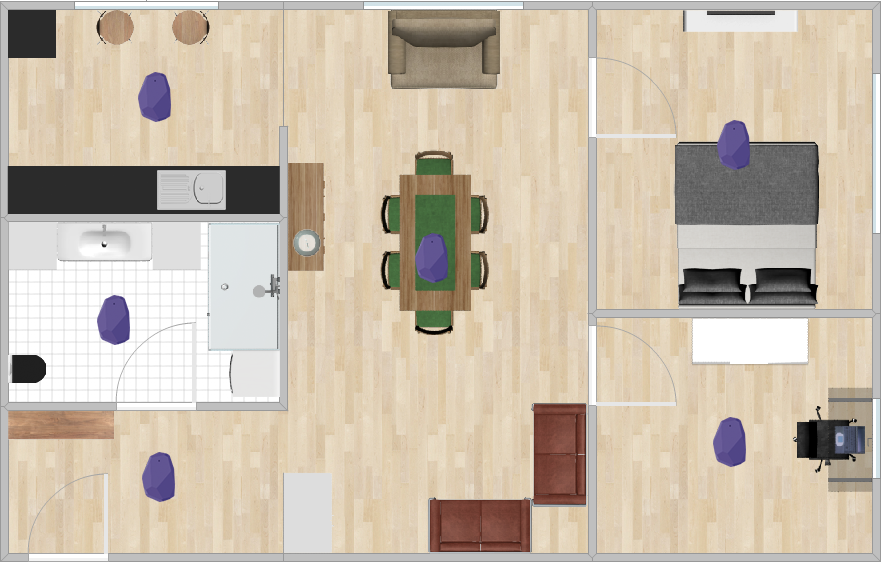
\includegraphics[width=\textwidth]{images/room-with-beacons}
\label{fig:analysis:scenario:apartment}
\caption{Example apartment we envision the system to be installed in.}
\end{figure}

We consider the following example of a day in a users life realistic to take place in the apartment illustrated in \Cref{fig:analysis:scenario:apartment,tbl:analysis:scenario:rooms} with the gestures outline in \Cref{tbl:analysis:scenario:gestures}.

\begin{testexample}
At the begnning of the day, the user wakes up in his bedroom. He makes a Z gesture to turn on Lamp 8 in the bedroom and gets out of bed. He goes to the bathroom to take a shower and turns on Lamp 12 by performing gesture Z as he enters. When he is done, he performs gesture Z to turn off the Lamp 12.

The user goes into the living room, and increases the temperature by performing gesture L, turns on Lamp 4 and Lamp 5 by performing gestures V and Triangle. Before he goes to the kitchen, he starts the music in the living room by performing the Circle gesture. In the kitchen he starts brewing coffee by performing the W gesture and gets some breakfast.

When the user is done eating breakfast, he goes to the living room and turns off the music by performing the Circle gesture. The user goes to the home office, starts the music in the office by performing the Circle gesture and turns on Lamp 10 and Lamp 11 by performing gestures Z and V.

When done working, he goes grocery shopping. As he leaves the home office, he performs gestures Z and V to turn off Lamp 10 and Lamp 11. He goes to the hallway and performs the Circle gesture to unlock the door. The user locks the door by performing a Circle gesture.

When the user comes home, he unlocks the door by performing a Circle gesture and unpacks his groceries in the kitchen in which he turns on Lamp 7 by performing a V gesture. Whe he is done unpacking the grocieries, he turns off Lamp 7 again by performing the V gesture again.

Earlier that day, the user had turned on Lamp 4 and Lamp 5 in the living room. He goes to the living room and turns off Lamp 4 and Lamp 5 by performing the V and Triangle gestures. He continues to the bedroom to watch television. The television is turned on by performing the Circle gesture. After watching television, the user turns off the TV by performing the Circle gesture and Lamp 8 by performing the Z gesture.
\end{testexample}

The above example briefly shows how the user can move around his apartment and use the same eight gestures to control different devices located in different rooms.

\subsection{Handling Uncertainties}
\label{sec:analysis:scenarios:handling_uncertainties}

Not all scenarios will work out as well as the one previously presented.
Sometimes a meaningful action cannot be determined from a gesture or the context of the user.
Assume that a person is in his living room and he performs a gesture that is recognized as ``Turn on TV'', but the only TV in the house (located in the living room) is already turned on.
In this case the action could be considered void, but we propose a different solution.
Rather than just ignoring the persons request, a list of alternate actions could be presented to him on his smartwatch.

It may be safe to assume that the person wanted to interact with the TV if the gesture performed was bound to this device, thus the target is still determined from the gesture, the location of the user and the location of the device, just as in the previous scenario.
Which actions would be presented however, could be the inverse of the one performed (if applicable) which in this case would be to turn the TV off.
It could also be a list of the actions most frequently performed by the user.

Another case of uncertainty would be if the gesture performed was not recognized.
This could be considered void and the person would be asked to try again, or the intended target could be assumed to be the device that the person most recently interacted with, and a list of the most frequently used actions could be presented on the persons watch.

\subsection{Controlling Devices in Other Rooms}
\label{sec:analysis:scenarios:other_rooms}

Assume that a person is in his home office listening to music but then remembers that he forgot to turn off the music in the living room.
He wishes to turn off the music in the living room but not the one located in the home office.
If the user performs the Circle gesture to pause the music, he would pause it in the home office.
To circumvent this, the smartwatch application could allow the user to select which room he would like to control devices in.

%%% Local Variables:
%%% mode: latex
%%% TeX-master: "../../master"
%%% End:
